\begin{center}
    \textit{Heaven’s Light is Our Guide} \\
    \vspace{1cm}
    \Large{Rajshahi University of Engineering \& Technology} \\
    \vspace{1cm}
    
\includegraphics[width=3cm]{ruet-logo.png}\\
    \vspace{0.1cm}
    \Large{Department of Computer Science and Engineering} \\
    \vspace{1cm}
    \large{\textbf{Course no:} CSE 4204} \\
    \large{\textbf{Course Title:} Sessional Based on CSE 4203} \\
    \large{\textbf{Experiment no:} 2}\\
    \large{\textbf{Name of the experiment:}} \\
    \large{Design and implementation of single layer
    perceptron learning algorithm.} \\
    \vspace{1cm}
\end{center}
\thispagestyle{empty}
\Large{\textbf{Submitted by}}\\
Partho Kumar Rajvor \\
Roll: 1803119 \\
Section: B \\
Department of Computer Science and Engineering\\
Rajshahi University of Engineering and Technology\\\\
\Large{\textbf{Submitted to}}\\
Rizoan Toufiq \\
Assistant Professor \\
Department of Computer Science and Engineering \\
Rajshahi University of Engineering and Technology
\tableofcontents

\setcounter{chapter}{1}
\chapter{Design and implementation of single layer
perceptron learning algorithm.}
\section{Introduction}
The perceptron is an algorithm for supervised learning of binary classifiers. A binary classifier is a function which can decide whether or not an input, represented by a vector of numbers, belongs to some specific class. It is a type of linear classifier, i.e. a classification algorithm that makes its predictions based on a linear predictor function combining a set of weights with the feature vector. The algorithm allows for online learning, in that it processes elements in the training set one at a time.\\

\section{About the dataset}
In this lab, we will be using the same dataset as we used in the previous lab.\\
\subsection{Foreword}
We will be using the following libraries in this lab:
\begin{itemize}
    \item \textit{pandas} for loading and preprocessing the dataset.
    \item \textit{scikit-learn} for splitting the dataset into training and test sets and for implementing the k-NN algorithm as well as for calculating the accuracy of the model.
\end{itemize}
\subsection{Preprocessing the dataset}
To ease the process of working with the dataset, we will specifically preprocess the \textit{disagnosis} column of the dataset. We will replace the values \textit{M} and \textit{B} with 1 and 0 respectively. This will help us to work with the dataset more easily.
\begin{lstlisting}[language=Python]
    df['diagnosis'] = df['diagnosis']
                        .replace('M', 1)
    df['diagnosis'] = df['diagnosis']
                        .replace('B', 0)
\end{lstlisting}
\subsection{Selecting the features and the output}
We will be using the first 30 columns of the dataset as the features and the last column as the output. We will use the following code snippet to select the features and the output:
\begin{lstlisting}[language=Python]
    x = df.iloc[:, 2:32]
    y = df.iloc[:, 1]
\end{lstlisting}
\section{Implementing the Perceptron algorithm}
\subsection{Algotihm of the Perceptron}
\begin{enumerate}
    \item Initialize the weights to 0 or small random numbers.
    Define $w_i$(t), ($i = 1, 2, ..., n$) as the weight vector at time $t$. And $\theta$ as the threshold. Set $w_0$(t) = -$\theta$, and $x_0$ = 1.
    Set $w_i(0)$ = some small random number.
    \item Present input and desired output patterns.
    \item Calculate actual output.
    y(t) = $f_h$[$\sum_{i=0}^{n} w_i(t)x_i(t)$]
    \item Adapt weights:\\\\
    \textbf{Using naive rule}\\
    if correct output, do nothing.\\
    ie, $w_i(t+1)$ = $w_i(t)$\\
    if output is 0, should have been 1, $w_i$(t+1) = $w_i$(t) + $x_i$(t)\\
    if output is 1, should have been 0, $w_i$(t+1) = $w_i$(t) - $x_i$(t)\\\\
    \textbf{Using modified rule}\\
    if correct output, do nothing.\\
    ie, $w_i(t+1)$ = $w_i(t)$\\
    if output is 0, should have been 1, $w_i$(t+1) = $w_i$(t) + $\eta x_i$(t)\\
    if output is 1, should have been 0, $w_i$(t+1) = $w_i$(t) - $\eta x_i$(t)\\
    where $\eta$ is the learning rate that ranges from 0 to 1.\\\\
    \textbf{Using delta rule}\\
    $\Delta$ = $d(t)$ - $y(t)$\\
    if correct output, do nothing.\\
    ie, $w_i(t+1)$ = $w_i(t)$\\
    if output is 0, should have been 1, $w_i$(t+1) = $w_i$(t) + $\eta \Delta x_i$(t)\\
    if output is 1, should have been 0, $w_i$(t+1) = $w_i$(t) - $\eta \Delta x_i$(t)\\
    where $\eta$ is the learning rate that ranges from 0 to 1.\\\\
\end{enumerate}
\subsection{Implementing the algorithm}
\begin{lstlisting}[language=Python]
class Perceptron:
    def __init__(self, 
                bias, 
                adaption_rate=0.01, 
                n_epochs=100, 
                adaption_method=None):
        self.ar = adaption_rate
        self.n_epochs = n_epochs
        self.activation_func = 
        lambda arr: 
                    np.where(arr > 0, 1, 0)
        self.weights = None
        self.bias = bias
        self.adaption_method = adaption_method

    def fit(self, X, y):
        # prepend 1 to X
        X = np.insert(X, 0, 1, axis=1)
        # assign random weights
        self.weights = np.random.rand(X.shape[1])
        # adjust w0
        self.weights[0] = -self.bias
        for _ in range(self.n_epochs):
            for idx, x_i in enumerate(X):
                y_hat = self.activation_func(
                    np.dot(x_i, self.weights)
                    )
                # adapt weights
                if self.adaption_method is None:
                    if y_hat == 0 and y[idx] == 1:
                        self.weights += x_i
                    elif y_hat == 1 and y[idx] == 0:
                        self.weights -= x_i
                elif self.adaption_method 
                == 'modified':
                    if y_hat == 0 and y[idx] == 1:
                        self.weights += self.ar*x_i
                    elif y_hat == 1 and y[idx] == 0:
                        self.weights -= self.ar*x_i
                elif self.adaption_method == 'delta':
                    delta = y[idx] - y_hat
                    self.weights +=
                     self.ar * delta * x_i

    def predict(self, X):
        # prepend 1 to X
        X = np.insert(X, 0, 1, axis=1)
        return self.activation_func(
            np.dot(X, self.weights)
        )
\end{lstlisting}
\subsection{Splitting the dataset into training and test sets}
We will be using the \textit{scikit-learn} library to split the dataset into training and test sets. We will use the following code snippet to split the dataset into training and test sets:
\begin{lstlisting}[language=Python]
    X = df.iloc[:, 2:32]
    y = df.iloc[:, 1]
    X_train, X_test, y_train, y_test = 
    train_test_split(X, y, test_size=0.2)
    X_train = np.array(X_train)
    X_test = np.array(X_test)
    y_train = np.array(y_train)
    y_test = np.array(y_test)
\end{lstlisting}
\section{Training the model}
\subsection{Initialize $w_i$(0)}
\begin{lstlisting}[language=Python]
    weights = np.random.rand(X.shape[1] + 1)
\end{lstlisting}
\subsection{Training the model using \\the naive rule}
\begin{lstlisting}[language=Python]
p = Perceptron(weights=weights, 
               bias=1.5)
p.fit(X_train, y_train)
y_pred = p.predict(X_test)
\end{lstlisting}
\subsection{Accuracy of the model}
We will use the following code snippet to calculate the accuracy of the model:
\begin{lstlisting}[language=Python]
acc = accuracy_score(y_test, y_pred)
print(f'Accuracy: {acc}')
cm = confusion_matrix(y_test, y_pred)
print(f'Confusion Matrix:\n{cm}')
f1 = f1_score(y_test, y_pred)
print(f'F1 Score: {f1}')
\end{lstlisting}
\textbf{Output:}\\
Accuracy: 0.8596491228070176\\
$$
\begin{bmatrix}
74 & 0 \\
16 & 24
\end{bmatrix}
$$\\
F1 Score: 0.7499999999999999
\subsection{Training the model using \\the modified rule}
\begin{lstlisting}[language=Python]
p = Perceptron(weights=weights, 
               bias=.5, 
               adaption_method='modified')
p.fit(X_train, y_train)
y_pred = p.predict(X_test)
\end{lstlisting}
\subsection{Accuracy of the model}
We will use the following code snippet to calculate the accuracy of the model:
\begin{lstlisting}[language=Python]
acc = accuracy_score(y_test, y_pred)
print(f'Accuracy: {acc}')
cm = confusion_matrix(y_test, y_pred)
print(f'Confusion Matrix:\n{cm}')
f1 = f1_score(y_test, y_pred)
print(f'F1 Score: {f1}')
\end{lstlisting}
\textbf{Output:}\\
Accuracy: 0.9122807017543859\\
$$
\begin{bmatrix}
74 & 0 \\
10 & 30
\end{bmatrix}
$$\\
F1 Score: 0.8571428571428571
\subsection{Training the model using \\the delta rule}
\begin{lstlisting}[language=Python]
p = Perceptron(weights=weights, 
               bias=1.5, 
               adaption_method='delta')
p.fit(X_train, y_train)
y_pred = p.predict(X_test)
\end{lstlisting}
\subsection{Accuracy of the model}
We will use the following code snippet to calculate the accuracy of the model:
\begin{lstlisting}[language=Python]
acc = accuracy_score(y_test, y_pred)
print(f'Accuracy: {acc}')
cm = confusion_matrix(y_test, y_pred)
print(f'Confusion Matrix:\n{cm}')
f1 = f1_score(y_test, y_pred)
print(f'F1 Score: {f1}')
\end{lstlisting}
\textbf{Output:}\\
Accuracy: 0.9122807017543859\\
Confusion Matrix:
$$
\begin{bmatrix}
74 & 0 \\
10 & 30
\end{bmatrix}
$$\\
F1 Score: 0.8571428571428571

\section{Visualization of the results}
\subsection{Scatter plot using testing input and desired output}
We will be using two features to plot the scatter plot. We will use the following code snippet to plot the scatter plot:
\begin{lstlisting}[language=Python]
fig = plt.figure()
ax = fig.add_subplot(1, 1, 1)
plt.scatter(X_test[:, 0],
            X_test[:, 1],
            marker="o", c=y_test)
plt.show()
\end{lstlisting}
\begin{figure}[ht]
    \centering
    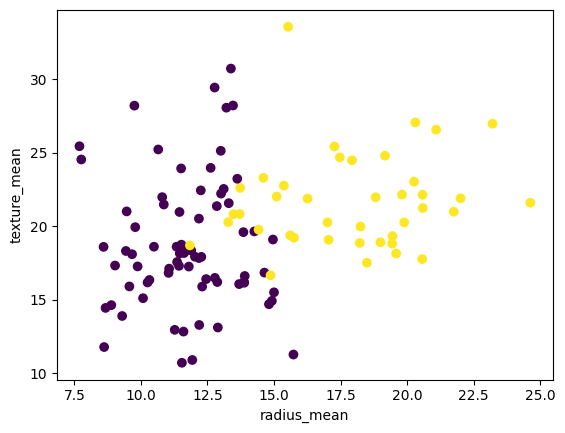
\includegraphics[width=10cm]{ch/figures/scatter1.png}
    \caption{Scatter plot using testing input and desired output}
    \label{fig:scatter1}
\end{figure}
\subsection{Scatter plot using testing input and predicted output}
We will be using two features to plot the scatter plot. Here we are using the prediction result from the delta rule.
\begin{lstlisting}[language=Python]
plt.scatter(X_test[:, 0],
            X_test[:, 1], 
            marker="o", 
            c=y_pred)
plt.show()
\end{lstlisting}
\begin{figure}[ht]
    \centering
    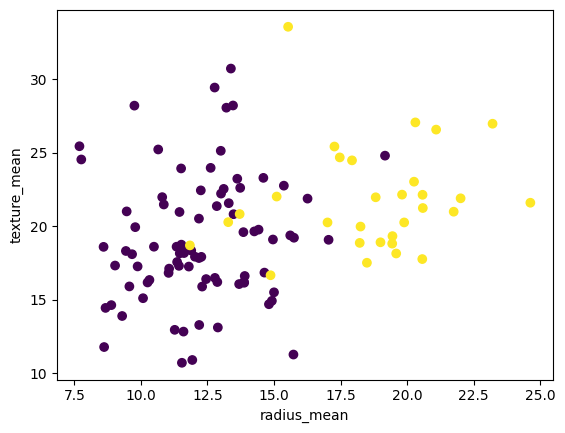
\includegraphics[width=10cm]{ch/figures/scatter2.png}
    \caption{Scatter plot using testing input and predicted output}
    \label{fig:scatter2}
\end{figure}
\section{Using the delta method to solve AND problem}
\subsection{Training the model}
\begin{lstlisting}[language=Python]
X = np.array([[0, 0], [0, 1], [1, 0], [1, 1]])
y = np.array([0, 0, 0, 1])
weights = np.random.rand(X.shape[1] + 1)
p = Perceptron(
weights, 
bias=1.5, 
adaption_method='delta')
p.fit(X, y)
y_pred = p.predict(X)
\end{lstlisting}
\subsection{Accuracy of the model}
\begin{lstlisting}[language=Python]
acc = accuracy_score(y, y_pred)
print(f'Accuracy: {acc}')
\end{lstlisting}
\subsection{Output}
Accuracy: 1.0

\section{Conclusion}
In this lab, we have implemented the Perceptron algorithm and used it to solve the breast cancer classification problem. We have also used the Perceptron algorithm to solve the AND problem. We have also visualized the results of the Perceptron algorithm.